	
\section{What is Emotion?}
	
\subsection{Definition}
	Wierzbicka argues emotions, such as anger, ``can be defined in terms of universal semantic primitives" (Wierzbick, 2003). A collection of semantic primitves, such as good or want, are used to rigidly define emotions such that emotions which are similar, such as happy and sad, appear as two distinctly defined emotions. Caband argues against this categorical definition of emotions and instead defines them by way of a common currency (Caband, 2002). Caband proposes that ``emotion is any mental experience" with high pleasure/displeasure, the common currency, and with high intensity. This definition places emotion in a scale rather than categories. A categorical approach to define and classify emotions is taken to simplify this project.

\subsection{Classifying Emotion}
	The classification of emotions has evolved over time. Ekman devised a list of well established emotions in 1972 after conducting experiments on multiple cultures, labeling data from facial expressions. Ekman's six emotions included anger, disgust, fear, happiness, sadness and surprise. Researches such as Sabini and Silver argued this list is incomplete, missing emotions such as love (Sabini \& Silver 2005). However, Ekman's contribution set a baseline for emotion classification built upon by future researchers.

	Plutchik aimed to categorize emotions less rigidly, creating the now popular representation ``wheel of emotion" (Plutchik 1982) seen in Figure \ref{fig:emotioncone}. He hypothesized emotions could blend together to define equivalence classes of emotions. With further research, he improved the wheel into a conic figure, factoring in parameters such as intensity. The four baseline emotional pairs used by Plutchik are illustrated in the figure. 
	
		\begin{figure}[!htb]
		\center{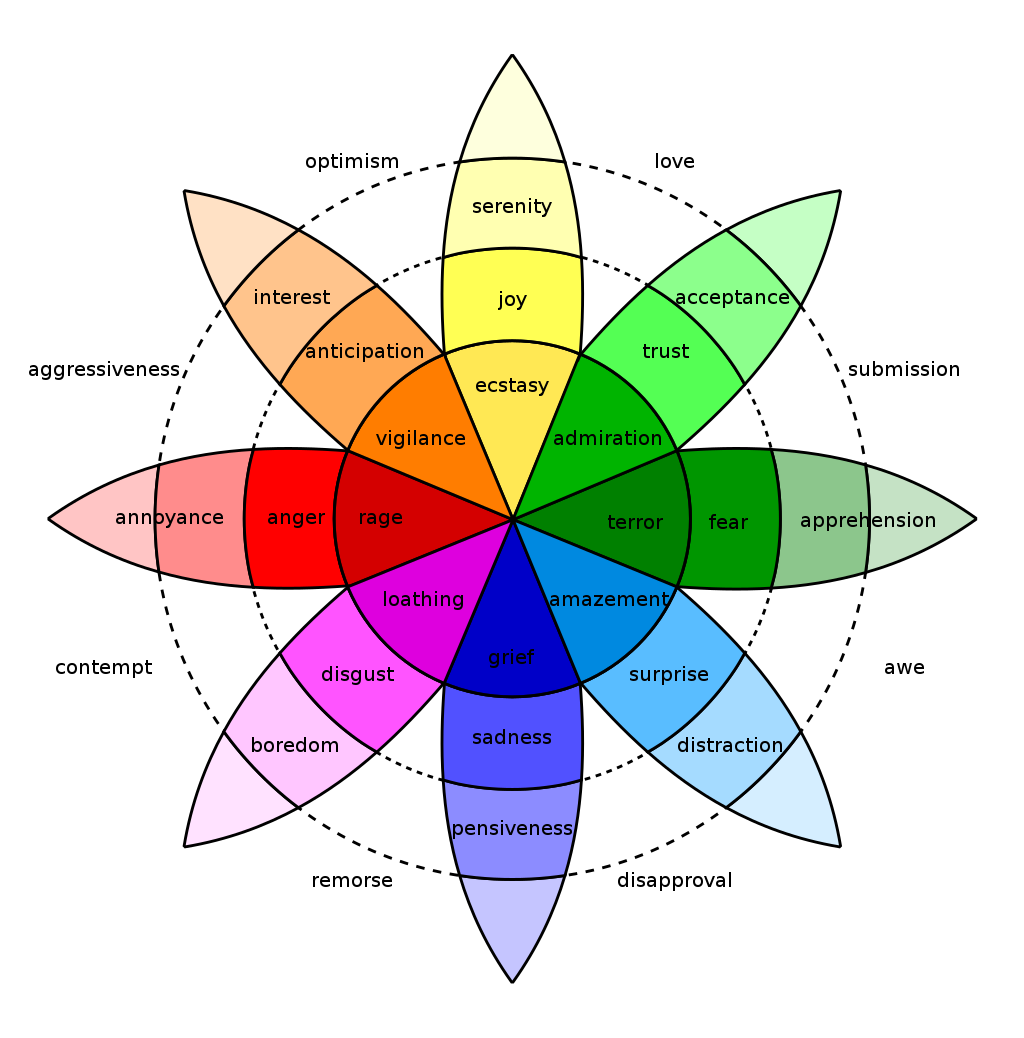
\includegraphics[width=8.5cm]
			{emotioncone}}
		\caption{\label{fig:emotioncone} Plutchik's Wheel of Emotion}
	\end{figure}

	Parrot proposed emotion can be classified in a tree structure. Primary emotions encompass a set of Secondary emotions that break down to a set of Tertiary emotions. The structure removes any connection between emotions of a different category. For example, Love and Joy, and all emotions derived from them, are not connected in any way (Parrot 2001). Parrot defines emotions distinctly, like Ekman, rather than using a scale, like Plutchik. Unlike Ekman's categorization, Parrot's is more nuanced. Automatic emotion recognition tasks become simpler when using distinct definitions.
	
	Research in determining distinct classes of emotion is still ongoing. Using reports of emotional states elicited by videos varying in emotional content, researchers (Cowen \& Keltner 2017) observed 27 varieties of emotion. ``Although categories are found to organize dimensional appraisals in a coherent and powerful fashion, many categories are linked by smooth gradients, contrary to discrete theories."
	
\subsection{Applications}
	Automatic Emotion Recognition has many practical applications ranging from Human Computer Interaction to military training. (Landowska et. al 2014) describe uses in the domains of ``software engineering, website customization, education, and gaming" in detail. Customizing websites and video games to respond to a user's emotional state can improve the user's experience by adapting to said responses. Understanding how people in education react to scenarios, such as exams, can help in improving education on an individual basis by giving a clearer profile for improvement.
	
	A key example, monitoring soldier emotion during training provides concrete feedback when attempting to emulate real world stressful situations. Understanding the emotional engagement of soldiers in training better prepares them for the real situation they are training for. The emotional feedback can be used to reduce the impact of Post Traumatic Stress Disorder and to improve already existing PTSD therapy. (Rizzo et. al 2005)
	
\subsection{Automatic Emotion Recognition}
	Automatic Emotion Recognition can be done using text, facial expressions and gestures, audio or a mixture of them (Seal et. al 2019). Text based recognition uses semantic labels to classify emotions. With images and videos, gestures and facial expressions are used to classify emotions. Speech data can be used as both its own set of features and as transcribed text with speech recognition to apply text-based emotion recognition. This paper aims to use acoustic speech data for automatic emotion recognition without any text based approach.

\section{Emotion Recognition from Speech}
	Speech Recognition is the most common form of speech technology. However, there are more speech technologies that relay a different set of information than recognition; verification, to identify a speaker, emotion recognition, to classify emotions, and synthesis, to generate speech. Speech recognition is often concerned with the phones corresponding to letters, words and phrases and suffers in performance due to differences in the voice patterns of individuals. On the other hand, verification and identification focuses on identifying the speaker through their unique patterns. Despite our understanding of the differences, research proves features designed for one task can find similar success with other tasks (Mackova et. al 2016). Most of the signal processing and feature extraction is similar between the forms of speech technologies despite the different aims of each.
	
\subsection{Data Collection}
	Emotion Recognition faces immediate problems from data collection and labeling. For example, Emotions are not equally defined across different cultures (Mesquita \& Walker 2003). "Cultural differences exist in some aspects of emotions," so difficulties exist when perceiving emotion expressed from a person raised in a different culture than the recognizer (Lim 2016). There is evidence to the claim of emotional recognition being more universal in facial recognition and gestures (Lorette \& Dewaele 2018, Matsumoto \& Hwang 2019), however speech and language still suffers from cultural and language differences.
	
	Mislabeling of emotion is not limited to cultural differences. Instances exist of humans not agreeing on identifying an emotion (Yarnell et. al 2017). While this issue is not as prevalent in a scale or currency based definition for emotion, the simpler discrete classes will produce mislabeling if not enough classes are used in labeling, as demonstrated by (Cowen \& Keltner 2017).
	
	A speech database's, or corpus's, method of collecting and labeling data is where these issues should be tackled. Each corpus aims to collect and label data authentically. When collecting emotion speech data, the emotion is ideally authentic and not acted out because if people have varying perception of emotion then their acting may not be true to the emotion expressed. Examples include the Interactive Emotional Children’s Speech Corpus (IESC-Child) wherein children converse with robots in a Wizard of Oz setting to "induce different emotional reactions" authentically (Avila-George et al 2019). IESC-Child is spoken Mexican Spanish; it is important to specify the language to identify cultural implications. Similarly, the PF Star and AIBO corpora elicit natural reaction from children by placing them in a controlled scenario (Russell 2006, Batliner et. al 2004). PF Star and AIBO are in English and German, respectively, adding to the variety of languages to experiment with language differences.

\subsection{Feature Extraction}
	Feature extraction is an integral process in automatic emotion recognition. Speech data features can be divided into two distinct categories; acoustic and linguistic. Acoustic features are dominantly used in speech emotion recognition (Jin et. al 2015). The usage and importance of linguistic features varies with the methods a corpus is created with; emotions acted out may not contain relevant linguistic data, but a candid corpus can provide more information to improve classifier performance (Batliner et. al 2011).
	
	Features for audio signals are usually extracted from smaller frames within the speech signal. In short periods of time, an audio signal can be considered invariant, so traditional signal processing techniques can be used. The usual size of the frame used for speech processing is 20ms to 30ms 20ms to 30ms  (Reddy \& Vijayarajan 2020). Instead of taking the frames as they are, windowing functions are applied to handle the edges of the signal frame to avoid abrupt changes. Hamming and Rectangular Windowing are two common functions used (Othman \& Riadh 2008).
\subsubsection{Acoustic Features}
	Acoustic features can be broken down into two general categories; prosodic and spectral. As observed by (Frick 1985), "emotions can be expressed prosodically...through a variety of prosodic features." Commonly used prosodic features include pitch, energy and duration. Prosodic features are also speaker-specific (Ben Alex et. al 2018), so feature vectors extracted are generally relative rather than absolute to minimize the error from the difference. 
	
	Spectral features are derived from the frequency domain of a signal. A cepstrum, the inverse of the logarithm of a spectrum, emphasises changes in its respective spectrum. Mel frequency cepstral coefficients (MFCCs) are the most common cepstral features extracted for use in speech systems. MFCCs were originally proposed for identifying monosyllabic words in continuously spoken sentences, yet they were proven to be useful in speaker verification and emotion recognition too (Gupta 2016). MFCCs aim to replicate human hearing on the assumption the "ear is a reliable speaker recognizer" (Alim \& Rashid 2017). The human ear detects differences in a smaller range of frequency clearer than larger frequency ranges. MFCCs accomplish this by applying a filters spaced linearly at low frequencies and logarithmically at high frequencies on a speech signal.
	
\subsubsection{Supervectors}
	An issue with using MFCCs as a feature for classification algorithms, such as support vector machines, is the potential for different speech segments to have varying lengths of feature vectors. One early solution researchers used was time-averaging utterances to equalize the feature vector size (Markel et. al 1977). Despite computation efficiency, this method resulted in poorer accuracy. The common trend to improve results was to use data-to-model matching for classification, such as by using Gaussian Mixture Models (Kinnunen \& Li 2010).
	
	Gaussian Mixture Models (GMMs) require a large amount of data to be effective for an emotion class (Hu et. al 2007). A Universal Background Model (UBM) can be used instead. UBMs are class independent GMMs, so data from all emotional classes can be used to compensate for the sparse data from distinct classes. A UBM can then be adapted into a class specific GMM using an adaption algorithm based on maximum a posteriori (MAP) criterion (Chen \& Chen 2016). The mean vectors of the adapted GMM form the GMM Supervector.
	
	   \begin{figure}[!htb]
		\center{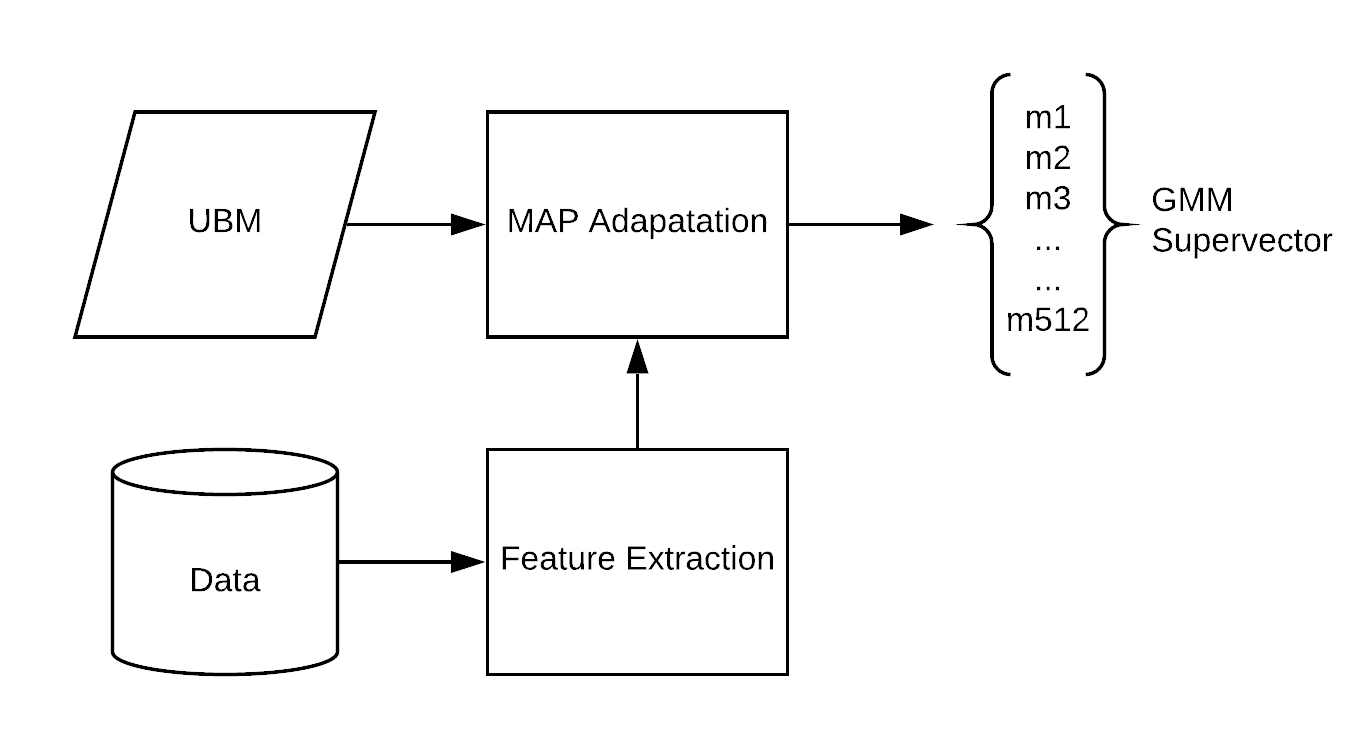
\includegraphics[width=11cm]
			{supervec}}
		\caption{\label{fig:supervec} Supervector Extraction Overview}
	\end{figure}

	Supervectors are a single vector representation of a GMM. Utterances with feature vectors of varying length can be converted into a standard length supervector by the process illustrated in Figure \ref{fig:supervec}. On one hand, a supervector solves both the issue of varying length features and reduced accuracy for use in classification algorithms. On the other hand, supervectors can be very high in dimension and computationally demanding.
\subsubsection{IVectors}
    I Vectors are a fixed length information rich low dimensional representation of a GMM-UBM based on Join Factor Analysis techniques originally proposed by (Dehak et. al 2010). I Vectors solve the issue of computational demand from supervectors while still having a standard size; they are at the forefront of research in speaker verification and emotion recognition from speech as demonstrated by the success found in experiments in speech recognition, speaker verification and emotion recognition (Karafiat et. al 2011, Mackova et. al 2016). The success can be attributed to it providing ``the benefit of modeling both the intra-domain and inter-domain variabilities into the same low dimensional space" (Ibrahim \& Ramli 2018).
\subsection{Classifiers}
	Automatic Emotion Recognition can be achieved using various machine learning and classification algorithms.
	SVMs are very commonly used for emotion recognition tasks and often exhibit the best performance (Chen \& Chen 2016, Mehta et. al 2019, Casale et. al 2008). This can be attributed to an SVMs robustness to high dimensional inputs such as the supervector (Han et. al 2014). GMM-UBM models are also used as classifiers rather than feature extractors, reaching performances upwards of 79\% (Schwenker et. al 2009).

	Deep learning methods are used most recently. Deep neural networks (DNNs) exhibit a number of improvements; they are capable of learning high-level representations from raw features to classify data (Han et. al 2014) and can function effectively on smaller data sets. Additionally, various architectures exists capable of handling data of different types. Convolutional Neural Networks (CNNs) have remarkable performance in n-dimensional vectors, such as images or layered features (Issa et. al 2020). Recurrant Neural Networks (RNNs) ``show considerable success" (Lim et. al 2014) in sequential data processing tasks, such as speech processing. Deep learning methods and hybrid neural networks have shown significant improvements in the relative range of 20\% accuracy increases (Han et. al  2014) compared to previous standards.
	
	Optimizing neural networks is required to improve the robustness and usability of an automatic emotion recognizer. (Batliner et. al 2004) achieved an overall recognition of 69.8\% using a neural network using a ``95 prosodic and 30 part-of-speech" features. (Xia \& Liu 2016) and (Heracleous \& Yoneyama 2019), and other researchers, convey the improvements of using I Vectors and neural network approach over earlier supervector and SVM techniques with their experimental results achievement results upwards of 90\%/.

